\chapter{Error de representación de datos}
\label{apendice-error}

La implementación del diseño de control en la placa de desarrollo fue limitada por las restricciones en las capacidades que presenta la Nexys 3 y su FPGA Spartan-6. Esta placa de desarrollo (y la gran mayoría de las FPGAs) no permite la síntesis a hardware de código con representación por punto flotante (indicado en VHDL con el tipo de dato llamado \texttt{real}), y por lo tanto era necesario utilizar la representación de los datos por punto fijo. Por una cuestión de balance entre cantidad de recursos usados y precisión, se eligió utilizar palabras de 32 bits.

Para los filtros digitales, debido a que los valores de entrada eran enteros de 0 a 4095 y los coeficientes del filtro no eran demasiado pequeños, se optó por una representación con 16 bits para la fracción, lo cual resultó ser una cantidad de bits suficiente para el funcionamiento de este componente.

Para el controlador proporcional-integral de corriente, la misma distribución de bits fue programada. La salida de este bloque se encuentra directamente conectada con el bloque generador de la señal de ancho de pulso modulado, el cual recibe un valor de 0 a 4095, y genera una señal PWM con el ciclo de trabajo acorde (es decir, posee una resolución de 12 bits). Como consecuencia, los coeficientes del controlador PI del lazo interno de corriente fueron escalados para asegurar que un valor unitario de ciclo de trabajo (100\%) se traduzca en una salida con valor 4095. Este escalamiento permite una asignación más flexible de la cantidad de bits para la parte fraccionaria, mientras se tenga en cuenta que obligatoriamente 12 bits son necesarios para la parte entera.

Sin embargo, el controlador PI del lazo externo de tensión no funciona de manera correcta utilizando la asignación mencionada en los bloques anteriores. Debido a que el cálculo de la acción de control por parte de este componente es a un valor `real', y los coeficientes del controlador son divididos por la frecuencia de muestreo (de \SI{625}{\kilo\hertz}), es necesaria una mejor resolución fraccionaria. En la Figura \ref{error-datos} puede apreciarse la simulación en Simulink\textsuperscript\textregistered\hspace{0.6pt} de la tensión de carga y la acción de control de tensión para 32 bits de palabra con 16 bits para la parte fraccionaria, y 24 bits para la parte fraccionaria.

\begin{figure}[hbt!]
    \centering
    \subfloat[Tensión de carga.\label{error-datos-tension}]{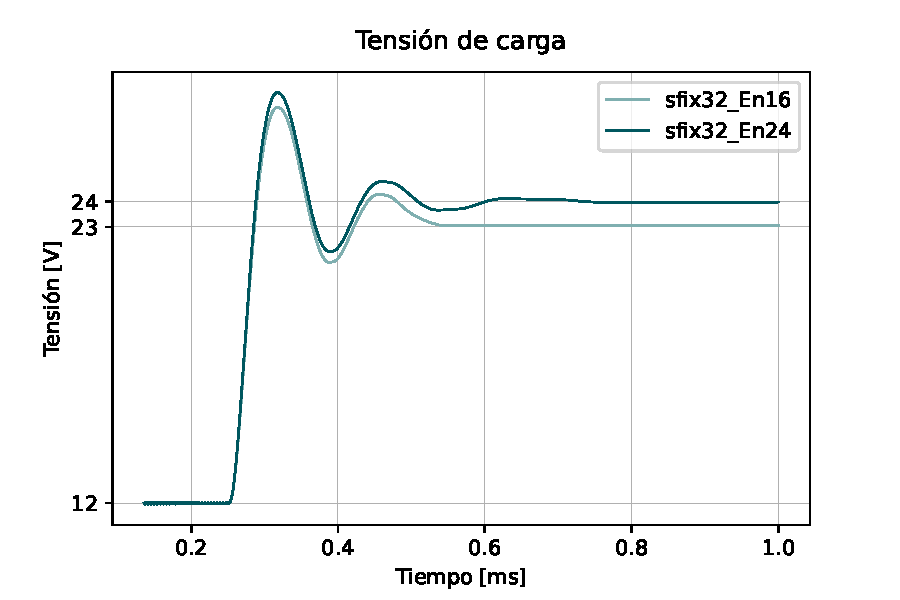
\includegraphics[width=0.45\textwidth]{Imágenes/Error de representación de datos/Tensión de carga.pdf}}    
    \subfloat[Acción de control de tensión.\label{error-datos-accion}]{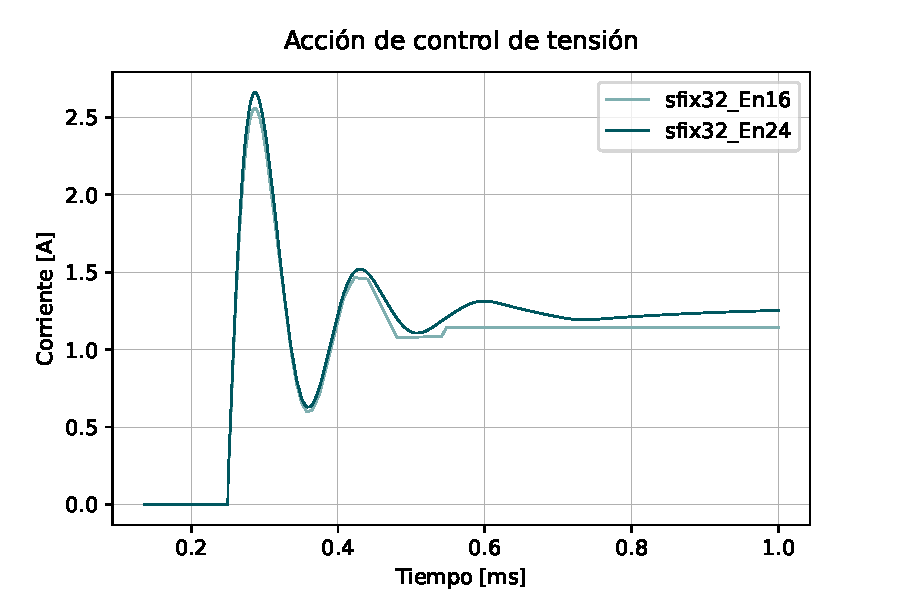
\includegraphics[width=0.45\textwidth]{Imágenes/Error de representación de datos/Acción de control de tensión.pdf}}
    \caption{Acción de control y tensión de carga con distinta distribución de cantidad de bits para representación de punto fijo.}
    \label{error-datos}
\end{figure}

Con representación de 16 bits para la fracción, se observa que la tensión de carga no se establece en el valor impuesto por la referencia, si no que ocurre un pequeño \emph{offset}. Esto es debido a que esta configuración de representación de datos no posee la resolución necesaria para generar una acción de control acorde con la tensión de referencia impuesta. Sin embargo, reasignando otros 8 bits más para la fracción es suficiente para que la acción de control genere una respuesta y un valor de estado estacionarios correctos. 

Otro problema presente en la representación de datos es el llamado \emph{integer overflow}. Este `desbordamiento' ocurre cuando una operación aritmética intenta crear un valor numérico afuera del rango posible del tipo de representación establecido. En VHDL, un \emph{integer overflow} resulta en el `envolvimiento' del valor almacenado, lo que significa que el valor almacenado en el caso de un desbordamiento es cero.

Debido al uso de integradores en los controladores del algortimo de control, el \emph{integer overflow} debe ser tenido en cuenta. La integración puede rápidamente causar un resultado que el tipo de datos elegido no es capaz de representar. En la Figura \ref{overflow} puede observarse para el caso del controlador PI de corriente cómo se presenta el desbordamiento. Aquí, se grafican la salida (de 0 a 4095, conectada al bloque generador de señal PWM) y el componente integrador del controlador. Se observa que el valor de la parte integral llega a 32768, y luego se produce un `overflow', lo cual hace que el dato se `envuelva' y llegue a -32768. Esto hace que la acción de control calculada se anule por la fuerte acción integral, la cual está incorrectamente representada.

\begin{figure}[hbt!]
    \centering
    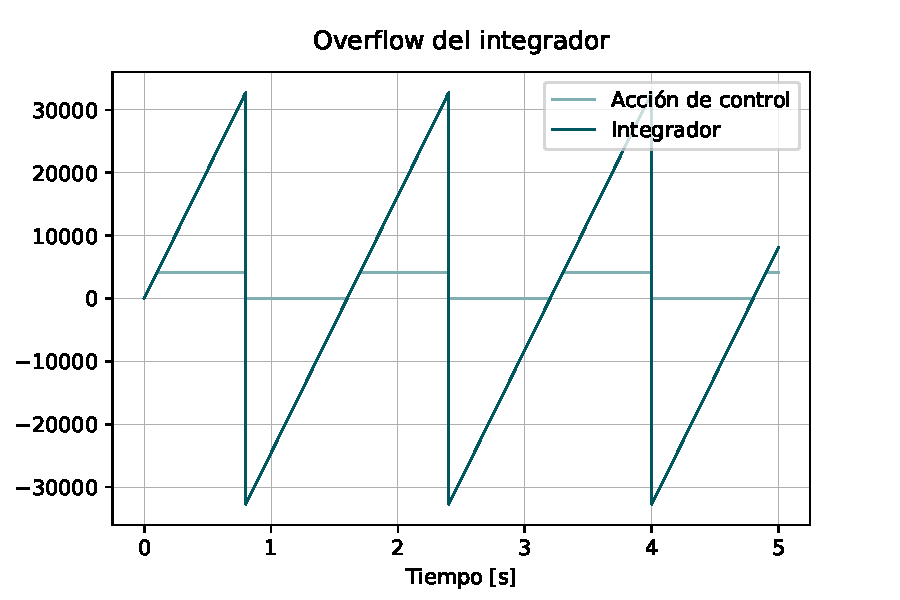
\includegraphics[width=0.50\columnwidth]{Imágenes/Overflow del integrador/Overflow del integrador.pdf}
    \caption{Overflow del integrador y su impacto en la acción de control.}
    \label{overflow}
\end{figure} 

Para evitar el desbordamiento de datos es necesario indicar al algoritmo, mediante un condicional, que la integración se detenga si el valor almacenado es el máximo posible de representar por el tipo de datos. Casualmente, este mismo método es utilizado para el diseño del controlador PI y es llamado \emph{clamping}. En la Figura \ref{clamping} se observa que al saturarse el integrador, se mantiene de esta manera sin ocurrir un desbordamiento.

\begin{figure}[hbt!]
    \centering
    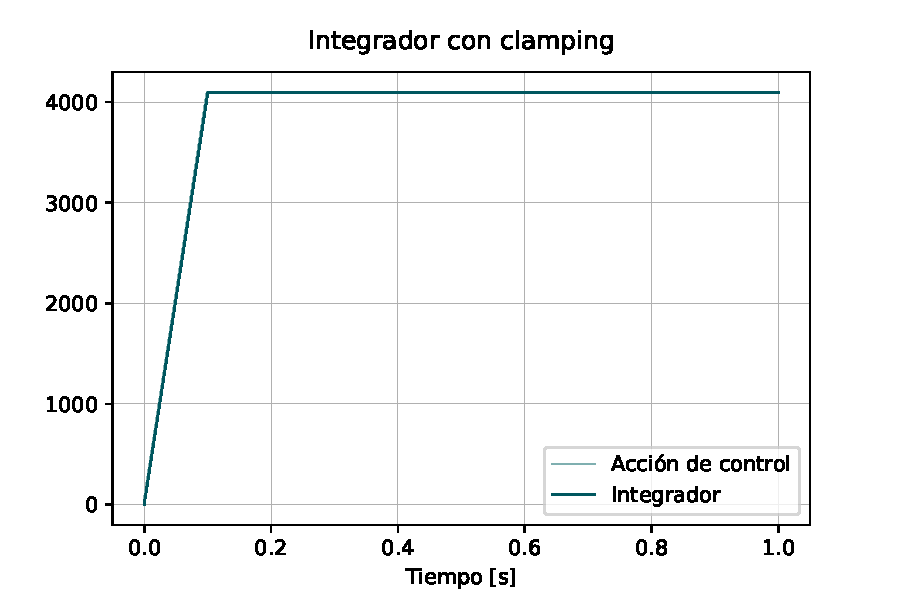
\includegraphics[width=0.50\columnwidth]{Imágenes/Overflow del integrador/Integrador con clamping.pdf}
    \caption{Integrador y acción de control con clamping.}
    \label{clamping}
\end{figure} 

\newpage